% =====================================================================
\section{Fase de Inicialización}
\label{sec:inicializacion}

En esta fase se preparó el entorno técnico, se definió la arquitectura del
sistema y se diseñó el modelo de datos, de modo que la fase de producción
pudiera concentrarse en la funcionalidad.

\subsection{Configuración del entorno de desarrollo}

La Tabla~\ref{tab:versiones} detalla las versiones de las tecnologías
instaladas, tomadas del archivo \archivo{package.json} del proyecto.

\begin{table}[H]
\centering
\caption{Versiones de las tecnologías utilizadas}
\label{tab:versiones}
\begin{tabularx}{\textwidth}{|L{5cm}|L{2.4cm}|Y|}
\hline
\rowcolor{encabezado} \textbf{Tecnología} & \textbf{Versión} & \textbf{Función} \\
\hline
Node.js & 22 & Entorno de ejecución de las herramientas \\ \hline
Expo SDK & 57 & Plataforma de desarrollo y módulos nativos \\ \hline
React Native / React & 0.86 / 19.2 & \emph{Framework} de interfaz \\ \hline
TypeScript & 6.0 & Lenguaje con tipado estático (modo estricto) \\ \hline
Expo Router & 57 & Navegación basada en archivos \\ \hline
Firebase JS SDK & 12 & Authentication, Firestore y Storage \\ \hline
NativeWind / Tailwind CSS & 4.2 / 3.4 & Estilos con clases utilitarias \\ \hline
Zustand & 5 & Estado global persistente \\ \hline
Zod & 4 & Validación de esquemas \\ \hline
react-native-chart-kit & 7 & Gráficos del reporte de progreso \\ \hline
expo-camera & 57 & Acceso a la cámara para el escáner \\ \hline
expo-image & 57 & Imágenes y animaciones GIF con caché \\ \hline
Google Sign-In (RN) & 16 & Inicio de sesión con Google \\
\hline
\end{tabularx}
\fuente{Archivo \archivo{package.json} del proyecto.}
\end{table}

Como la aplicación utiliza módulos nativos que no incluye Expo Go (inicio de
sesión con Google y cámara), se generó un \emph{development build} propio con
\archivo{npx expo run:android}, y se configuró el archivo \archivo{eas.json}
con los perfiles \emph{development}, \emph{preview} y \emph{production} para la
compilación en la nube.

\subsection{Repositorio y flujo de trabajo}

El código se versionó en un repositorio de GitHub con un flujo de ramas
inspirado en \emph{Git Flow} (Figura~\ref{fig:ramas}): la rama \archivo{main}
contiene las versiones estables, \archivo{develop} integra el trabajo en curso
y cada módulo se desarrolla en una rama \archivo{feature/*} que se incorpora a
\archivo{develop} mediante una solicitud de integración (\emph{pull request}).
Los mensajes de commit siguen la convención \emph{Conventional Commits}
(\archivo{feat}, \archivo{chore}, \archivo{build}), lo que permite leer el
historial por tipo de cambio.

\begin{figure}[H]
\centering
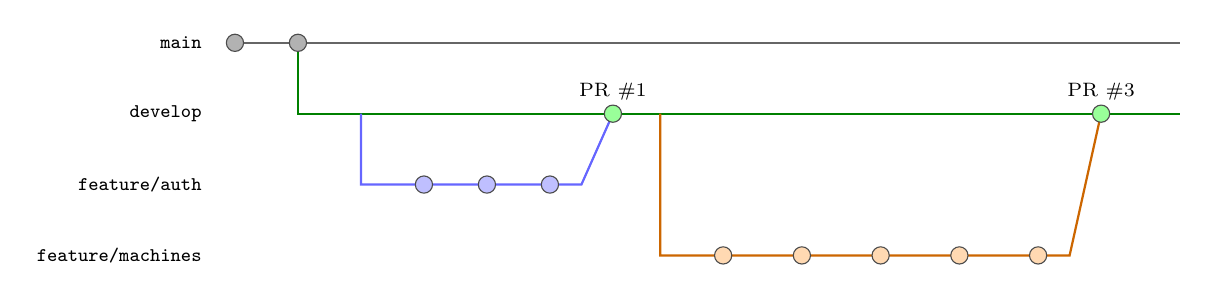
\begin{tikzpicture}[x=1cm, y=0.9cm,
  commit/.style={circle, draw=black!70, fill=#1, inner sep=2.2pt},
  rama/.style={font=\scriptsize\ttfamily, anchor=east}]
  \node[rama] at (-0.3,2) {main};
  \node[rama] at (-0.3,1) {develop};
  \node[rama] at (-0.3,0) {feature/auth};
  \node[rama] at (-0.3,-1) {feature/machines};
  \draw[thick, black!60] (0,2) -- (12,2);
  \draw[thick, green!50!black] (0.8,2) -- (0.8,1) -- (12,1);
  \draw[thick, blue!60] (1.6,1) -- (1.6,0) -- (4.4,0) -- (4.8,1);
  \draw[thick, orange!80!black] (5.4,1) -- (5.4,-1) -- (10.6,-1) -- (11,1);
  \foreach \x in {0,0.8} \node[commit=black!30] at (\x,2) {};
  \foreach \x in {2.4,3.2,4.0} \node[commit=blue!25] at (\x,0) {};
  \foreach \x in {6.2,7.2,8.2,9.2,10.2} \node[commit=orange!30] at (\x,-1) {};
  \node[commit=green!40] at (4.8,1) {};
  \node[commit=green!40] at (11,1) {};
  \node[font=\scriptsize, above] at (4.8,1.05) {PR \#1};
  \node[font=\scriptsize, above] at (11,1.05) {PR \#3};
\end{tikzpicture}
\caption{Flujo de ramas del repositorio}
\label{fig:ramas}
\fuente{Elaboración propia a partir del historial de Git del proyecto.}
\end{figure}

\subsection{Configuración de Firebase}

Se creó un proyecto en la consola de Firebase y se registró la aplicación
Android con su identificador de paquete. En él se habilitaron:

\begin{itemize}
    \item \textbf{Authentication}, con los proveedores de correo y contraseña
    y de Google.
    \item \textbf{Cloud Firestore}, para los datos de usuarios y el catálogo.
    \item \textbf{Cloud Storage}, para las imágenes y animaciones del catálogo.
\end{itemize}

Las claves de configuración se almacenan en un archivo \archivo{.env} con el
prefijo \archivo{EXPO\_PUBLIC\_}, excluido del control de versiones, y se leen
en un único módulo, \archivo{firebase.ts}, dentro de la carpeta de servicios. La sesión de
Firebase Authentication se persiste en el dispositivo con
\archivo{AsyncStorage}, de modo que el usuario no debe iniciar sesión cada vez
que abre la aplicación. Las claves de servicios de terceros que no deben
quedar dentro del paquete instalable, como la de WorkoutX, se usan únicamente
en los \emph{scripts} de carga que se ejecutan desde la computadora de
desarrollo.

\subsection{Arquitectura del sistema}
\label{subsec:arquitectura}

El sistema sigue una arquitectura cliente--servidor. El cliente es la
aplicación móvil, organizada internamente en capas según el patrón MVC; el
servidor está compuesto por los servicios administrados de Firebase y por la
API pública de wger (Figura~\ref{fig:arquitectura}).

\begin{figure}[H]
\centering
\begin{tikzpicture}[font=\small,
  lay/.style={rectangle, draw=black!60, fill=#1, minimum width=8.6cm,
    minimum height=1.25cm, align=left, text width=8.3cm, font=\footnotesize},
  srv/.style={rectangle, rounded corners=3pt, draw=black!60, fill=orange!8,
    minimum width=2.9cm, minimum height=0.95cm, align=center, font=\footnotesize}]
  % Cliente
  \node[lay=green!12] (vista) at (0,4.3) {\textbf{Vista} --- \archivo{app/}, \archivo{components/}\\
    Pantallas de Expo Router, componentes de interfaz, NativeWind};
  \node[lay=green!7] (ctrl) at (0,2.65) {\textbf{Controlador} --- \archivo{controllers/}, \archivo{utils/}, \archivo{store/}\\
    Casos de uso, reglas de negocio, generador de rutinas, estado global};
  \node[lay=green!4] (modelo) at (0,1.0) {\textbf{Modelo} --- \archivo{models/}, \archivo{schemas/}\\
    Entidades, esquemas Zod, repositorios (únicos que conocen Firestore)};
  \node[lay=black!4] (serv) at (0,-0.65) {\textbf{Servicios} --- \archivo{services/}\\
    Firestore, Storage, cliente HTTP de wger, punto de extensión de IA};
  \node[draw, dashed, rounded corners, fit=(vista)(serv), inner sep=8pt,
    label={[font=\small\bfseries]above:Cliente: aplicación Android}] (cli) {};
  \draw[flecha] (vista) -- (ctrl);
  \draw[flecha] (ctrl) -- (modelo);
  \draw[flecha] (modelo) -- (serv);
  % Servidor
  \node[srv] (auth) at (8.9,4.3) {Firebase\\Authentication};
  \node[srv] (fs) at (8.9,2.65) {Cloud\\Firestore};
  \node[srv] (st) at (8.9,1.0) {Cloud\\Storage};
  \node[srv, fill=blue!6] (wg) at (8.9,-0.65) {API REST\\de wger};
  \node[draw, dashed, rounded corners, fit=(auth)(wg), inner sep=8pt,
    label={[font=\small\bfseries]above:Servidor}] (sv) {};
  \draw[flecha, <->] (cli.east |- auth) -- node[above, font=\tiny]{SDK} (auth);
  \draw[flecha, <->] (cli.east |- fs) -- node[above, font=\tiny]{tiempo real} (fs);
  \draw[flecha, <->] (cli.east |- st) -- (st);
  \draw[flecha, <->] (cli.east |- wg) -- node[above, font=\tiny]{HTTPS} (wg);
\end{tikzpicture}
\caption{Arquitectura cliente--servidor y capas del cliente}
\label{fig:arquitectura}
\end{figure}

Las reglas de dependencia entre capas, que se respetaron en todo el código,
son las siguientes:

\begin{itemize}
    \item Las pantallas de \archivo{app/} son solo Vista: nunca importan
    Firebase ni contienen reglas de negocio; siempre llaman a un controlador.
    \item Los controladores validan los datos con Zod, aplican las reglas de
    negocio y coordinan a los repositorios.
    \item Los repositorios son el único lugar que conoce las rutas reales de
    Firestore (por ejemplo, \archivo{usuarios/\{uid\}/rutinas}).
    \item El SDK de Firestore solo se usa en \archivo{firestoreService.ts}, el
    de Storage solo en \archivo{storageService.ts} y el de Authentication solo
    en \archivo{AuthController.ts}.
\end{itemize}

\subsection{Estructura del proyecto}

El Código~\ref{lst:estructura} muestra la organización de carpetas del
código fuente y su correspondencia con las capas de la arquitectura.

\begin{lstlisting}[language={}, numbers=none, caption={Estructura de carpetas del código fuente}, label={lst:estructura}]
src/
  app/                    VISTA: rutas de Expo Router
    _layout.tsx           rutas protegidas segun sesion y perfil
    index.tsx             bienvenida
    (auth)/               LoginScreen, RegisterScreen
    (onboarding)/         TargetSelectionScreen, RoutineChoiceScreen
    (app)/                pestanas de la app autenticada
      index.tsx           inicio
      machines/           guia: index, [id] (ficha), escaner
      routines/           index, generar, personalizada
      nutricion.tsx       calculadora de IMC
      progress/           progreso y reporte
      perfil.tsx
  components/             VISTA: componentes reutilizables
  controllers/            CONTROLADOR: casos de uso por modulo
  utils/                  CONTROLADOR: generadorRutinas.ts, imcCalculator.ts
  store/                  estado global (Zustand): auth, onboarding
  hooks/                  suscripciones en tiempo real
  models/
    entities/             MODELO: tipos del dominio
    repositories/         MODELO: acceso a datos por coleccion
  schemas/                MODELO: validacion con Zod
  services/
    firebase/             SERVICIOS: Firestore y Storage
    wger/                 SERVICIOS: cliente HTTP de la API de wger
    ai/                   SERVICIOS: punto de extension de IA
  constants/              paleta de colores
\end{lstlisting}

\subsection{Modelo de datos}
\label{subsec:modelo-datos}

Cloud Firestore es una base de datos documental, por lo que el modelo se
diseñó a partir de los patrones de acceso de las pantallas y no de una
normalización relacional. Se aplicó una regla general: lo que es
\emph{catálogo} (compartido y de solo lectura) vive en colecciones raíz, y lo
que pertenece a un usuario vive en subcolecciones bajo su documento
(Figura~\ref{fig:modelo-datos}).

\begin{figure}[H]
\centering
\begin{tikzpicture}[font=\scriptsize]
  \node[entidad, anchor=north] (usr) at (0,1.2) {usuarios/\{uid\}
    \nodepart{second}nombre, apellidos, email\\genero, altura, pesoActual\\
    nivel, objetivo\\rutinaActivaId\\creadoEn, actualizadoEn};
  \node[entidad, anchor=north] (eje) at (-4.6,1.2) {ejercicios/\{id\}
    \nodepart{second}nombre, grupoMuscular[ ]\\descripcion\\
    seriesRecomendadas\\repeticionesRecomendadas};
  \node[entidad, anchor=north] (maq) at (6.7,1.2) {maquinas/\{id\}
    \nodepart{second}nombre, categoria, tipo\\orden, descripcion\\
    musculosPrincipales[ ]\\musculosSecundarios[ ]\\instrucciones[ ]\\
    erroresComunes[ ]\\prevencionLesiones[ ]\\imagenPrincipal\\gifPrincipal\\
    variantes[ ], ejercicios[ ]\\ejerciciosGif[ ]\\wgerIds[ ], workoutxIds[ ]};
  \node[entidad, anchor=north] (rut) at (-4.65,-2.0) {rutinas/\{id\}
    \nodepart{second}nombre, tipo\\objetivo, nivel\\
    diasPorSemana\\planSemanal[ ]\\usuarioId, creadoEn};
  \node[entidad, anchor=north] (nut) at (-0.85,-2.0) {registrosNutricionales/\{id\}
    \nodepart{second}weight, height\\bmi, category\\usuarioId, creadoEn};
  \node[entidad, anchor=north] (pro) at (2.85,-2.0) {progresoFisico/\{id\}
    \nodepart{second}peso, altura, imc\\notas\\usuarioId, creadoEn};
  \draw[thick] (usr.south) -- ++(0,-0.35) coordinate (bus);
  \draw[thick] (rut.north |- bus) -- (pro.north |- bus);
  \foreach \n in {rut,nut,pro} \draw[thick] (\n.north |- bus) -- (\n.north);
  \node[font=\scriptsize\itshape, anchor=west] at ($(bus)+(0.1,0.15)$) {subcolecciones privadas};
  \draw[flechad] (rut.south) -- ++(0,-0.45) -| node[pos=0.25, below, font=\scriptsize]{maquinaCatalogoId (opcional)} (maq.south);
  \node[font=\scriptsize\bfseries, above=2pt of maq] {Catálogo (solo lectura)};
  \node[font=\scriptsize\bfseries, above=2pt of eje] {Catálogo (solo lectura)};
  \node[font=\scriptsize\bfseries, above=2pt of usr] {Perfil del usuario};
\end{tikzpicture}
\caption{Modelo de datos en Cloud Firestore}
\label{fig:modelo-datos}
\end{figure}

Las decisiones de diseño más relevantes fueron:

\begin{itemize}
    \item \textbf{Subcolecciones por usuario.} Las rutinas, los registros
    nutricionales y el progreso físico cuelgan de
    \archivo{usuarios/\{uid\}}. El aislamiento entre usuarios queda expresado
    en la propia ruta, y las reglas de seguridad solo deben comparar ese
    segmento con el identificador del usuario autenticado. Además, cada
    documento conserva el campo \archivo{usuarioId} como defensa en
    profundidad.
    \item \textbf{El identificador del perfil es el \emph{uid}.} El documento
    \archivo{usuarios/\{uid\}} usa como clave el identificador de Firebase
    Authentication, lo que permite autorizar el acceso sin leer el documento
    previamente.
    \item \textbf{Marcas de tiempo del servidor.} Los campos
    \archivo{creadoEn} y \archivo{actualizadoEn} se generan con
    \archivo{serverTimestamp()} en la capa de servicios; nunca se construye
    una fecha en el cliente para persistirla.
    \item \textbf{Plan semanal embebido.} La rutina guarda su
    \archivo{planSemanal} como un arreglo de días, cada uno con su enfoque y
    sus ejercicios. Como una rutina siempre se lee completa y su tamaño es
    pequeño, embeber evita lecturas adicionales.
    \item \textbf{Rutas de Storage en lugar de URL.} Las fichas de las
    máquinas guardan la ruta del archivo en Storage (por ejemplo,
    \archivo{maquinas/prensa-piernas/principal.webp}); la URL de descarga se
    resuelve en tiempo de ejecución y se almacena en caché.
\end{itemize}

\subsection{Reglas de seguridad}

Las reglas de Firestore implementan el requerimiento RNF3. Definen dos
funciones auxiliares, \archivo{estaAutenticado()} y
\archivo{esDueno(usuarioId)}, y para cada subcolección validan la forma de los
datos. El Código~\ref{lst:regla-rutinas} muestra la regla de las rutinas; el
archivo completo, junto con las reglas de Storage, se incluye en el
Anexo~\ref{anx:reglas}.

\begin{lstlisting}[language=FirestoreRules, caption={Regla de seguridad de la subcolección de rutinas}, label={lst:regla-rutinas}]
match /rutinas/{rutinaId} {
  function rutinaValida() {
    let datos = request.resource.data;
    return datos.usuarioId == usuarioId
      && datos.nombre is string && datos.nombre.size() > 0
      && datos.tipo in ['ia', 'personalizada']
      && datos.diasPorSemana is number
      && datos.diasPorSemana >= 1 && datos.diasPorSemana <= 7
      && datos.planSemanal is list;
  }
  allow read, delete: if esDueno(usuarioId);
  allow create: if esDueno(usuarioId) && rutinaValida();
  allow update: if esDueno(usuarioId) && rutinaValida()
    && request.resource.data.usuarioId == resource.data.usuarioId;
}
\end{lstlisting}

El catálogo (\archivo{maquinas} y \archivo{ejercicios}) se declara con
\archivo{allow write: if false}. Su carga se realiza con el SDK de
administración de Firebase, que se autentica con una cuenta de servicio y no
está sujeto a las reglas de cliente, por lo que ningún usuario de la
aplicación puede modificarlo.

\subsection{Diseño de la navegación}

La navegación se diseñó con cuatro grupos de rutas, habilitados según el
estado de la sesión y del perfil (Tabla~\ref{tab:rutas-protegidas}). La
protección se implementa una sola vez en el diseño raíz con
\archivo{Stack.Protected}: cuando cambia el estado, Expo Router retira al
usuario de las pantallas que dejaron de estar disponibles y lo lleva a la
primera disponible, sin que ninguna pantalla deba redirigir manualmente.

\begin{table}[H]
\centering
\caption{Grupos de rutas habilitados según el estado}
\label{tab:rutas-protegidas}
\begin{tabularx}{\textwidth}{|Y|L{4.3cm}|}
\hline
\rowcolor{encabezado} \textbf{Estado} & \textbf{Grupo disponible} \\
\hline
Sin sesión & \archivo{index} (bienvenida) y \archivo{(auth)} \\ \hline
Con sesión, perfil aún cargando & \archivo{(auth)} \\ \hline
Con sesión, sin objetivo ni nivel & \archivo{(onboarding)} \\ \hline
Con sesión y perfil completo & \archivo{(app)} \\
\hline
\end{tabularx}
\end{table}

Dentro de \archivo{(app)}, la navegación principal es una barra de pestañas
con cuatro destinos: \emph{Inicio}, \emph{Máquinas}, \emph{Progreso} y
\emph{Nutrición}. Las rutinas y el perfil son rutas navegables desde el
inicio, ocultas en la barra para no sobrecargarla (RNF2).

\subsection{Sistema de diseño}

Para dar consistencia visual a la interfaz se definió una paleta de colores
centralizada en \archivo{global.css}, \archivo{tailwind.config.js} y
\archivo{constants/palette.ts}, consumida desde las pantallas con clases de
NativeWind (Tabla~\ref{tab:paleta}). El verde principal se asocia con salud y
actividad, y los tonos cálidos se reservan para acentos y alertas.

\newcommand{\muestra}[1]{\fcolorbox{black!40}[HTML]{#1}{\rule{0pt}{7pt}\hspace{0.8cm}}}
\begin{table}[H]
\centering
\caption{Paleta de colores de la aplicación}
\label{tab:paleta}
\begin{tabular}{|L{3.2cm}|C{1.4cm}|L{2.2cm}|L{5cm}|}
\hline
\rowcolor{encabezado} \textbf{Token} & \textbf{Color} & \textbf{Valor} & \textbf{Uso} \\
\hline
\archivo{primary} & \muestra{32A685} & \#32A685 & Botones, pestaña activa \\ \hline
\archivo{primaryLight} & \muestra{ADD9D1} & \#ADD9D1 & Bordes y superficies \\ \hline
\archivo{primaryDark} & \muestra{1F8A6A} & \#1F8A6A & Degradados \\ \hline
\archivo{secondary} & \muestra{F2C0A2} & \#F2C0A2 & Advertencias suaves \\ \hline
\archivo{accent} & \muestra{F29580} & \#F29580 & Acentos \\ \hline
\archivo{accentStrong} & \muestra{D95032} & \#D95032 & Errores y alertas \\ \hline
\archivo{foreground} & \muestra{1F2937} & \#1F2937 & Texto principal \\
\hline
\end{tabular}
\fuente{Archivo \archivo{constants/palette.ts} del proyecto.}
\end{table}

\subsection{Día de prueba}

La fase concluyó con el \emph{día de prueba} de Mobile-D, en el que se
verificó de extremo a extremo que la cadena de herramientas funcionaba: el
proyecto compiló sin errores de TypeScript, se generó el \emph{development build} para
Android, la aplicación se conectó a Firebase, se
publicaron las reglas de seguridad y los cambios se integraron en GitHub a
través de la rama \archivo{develop}. Con ello se dio por cerrada la
inicialización y se pasó a la fase de producción.
